\begin{figure*}[!t]
    \centering
    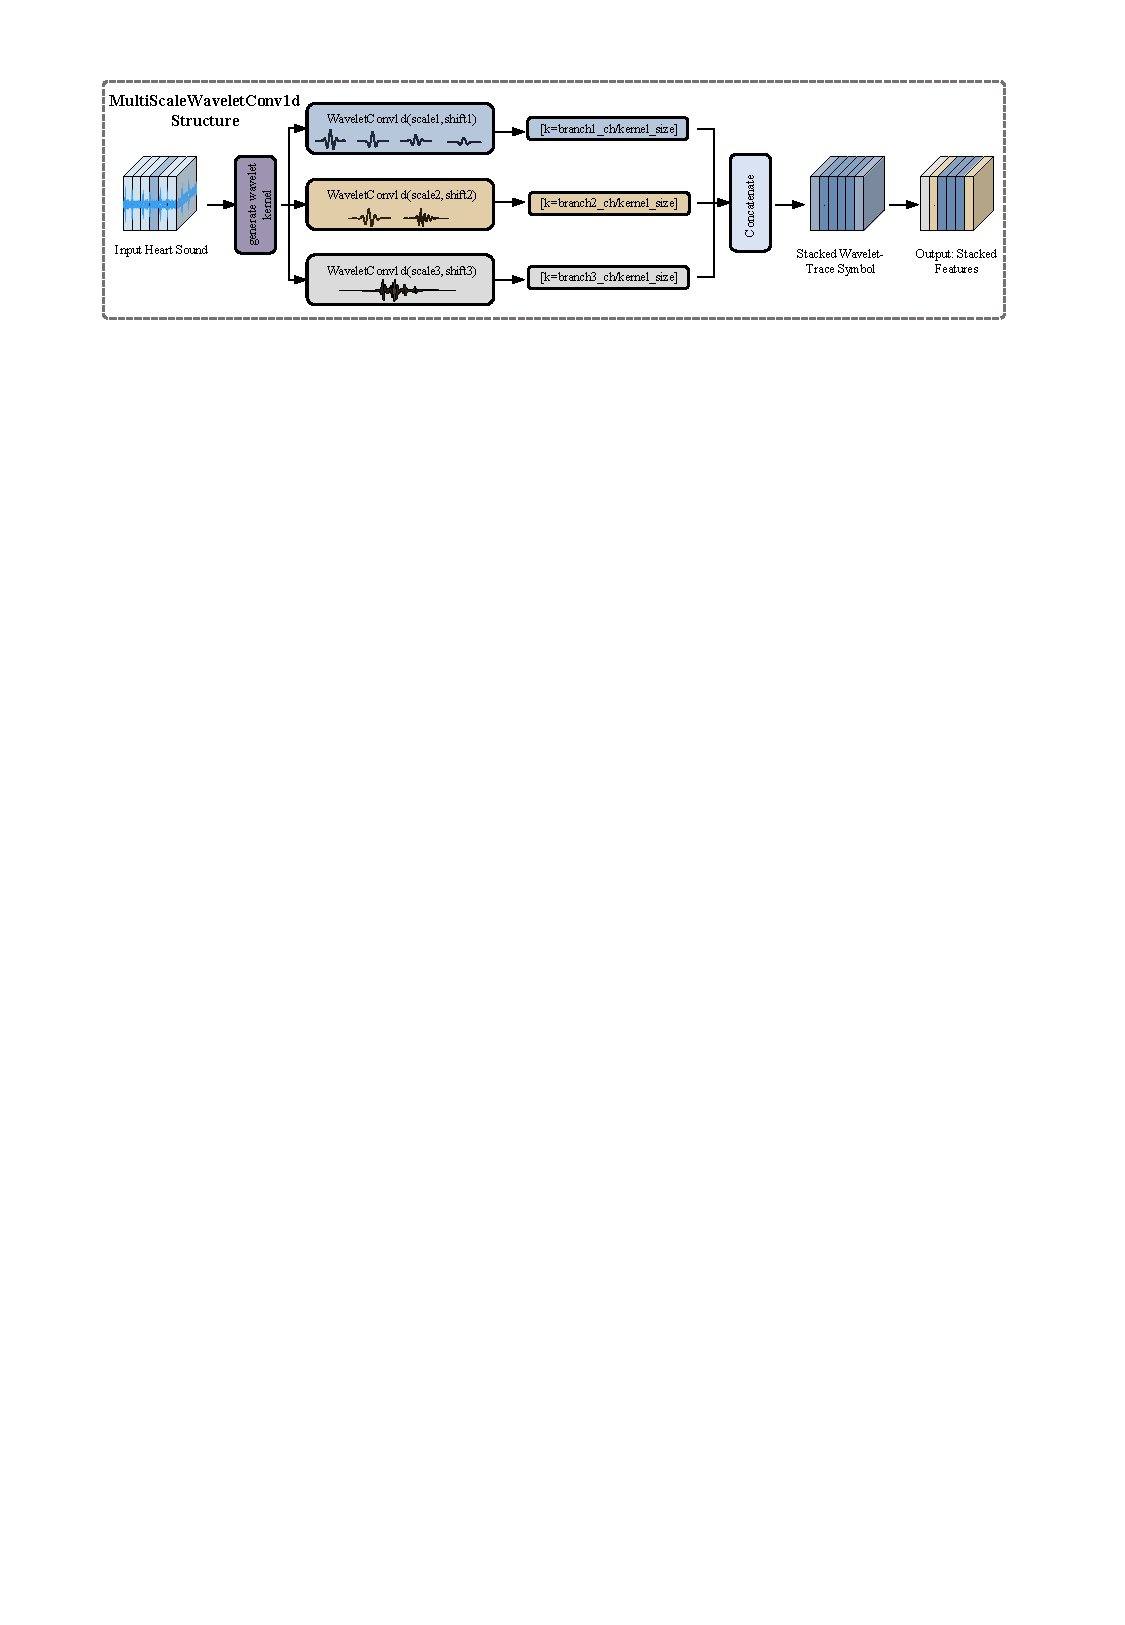
\includegraphics[width=.76\textwidth]{figures/MultiScaleWaveletConv1d Structure.pdf}
    \caption{\protect\re{Parallel-convolution core of MSWC. The ``generate wavelet kernel'' block denotes template-based initialisation. Three groups use nominal scale and shift settings, and their output features are concatenated along the channel dimension. The wavelet traces are schematic template symbols. Channel recalibration and feature enhancement are described in the text.}}
    \label{fig:mswc-structure}
\end{figure*}